\section{Simulation Studies}

\subsection{Simulation setup}

Data were generated and estimated using MPlus 8.4. Data-generating values are based on the real-data application of the models to the available subset of the data at the time of conducting the simulation study. That is, data were simulated for 40 individuals (N) observed across 9 or 12 measurement occasions, with 5 or 7 observed categories per indicator. 1000 replications were simulated. Data estimation took place using the MPlus default priors. In case of   LST models for one construct, default priors were compared with IG(0.001, 0.001) priors set on all variance parameters (model did not include latent covariances). Two chains with a minimum of 5,000 iterations per chain and a thinning factor of 10 was applied (i.e. at last 50,000 iterations of which only every 10th was used for constructing the posterior distribution). Convergence was assumed and estimation stopped when the PSR fell below 1.05 for the first time after the minimum number of iterations was reached.

\subsection{Summary of the results}

In the following, the 95\% coverage rate, the relative parameter estimation bias (deviation between average estimate and population parameter divided by the population parameter), the Mean Squared Error, absolute bias, as well as relative standard error bias are displayed for every simulated model. \\
Latent state models for one construct work well, with small biases (below a cutoff of 10\% bias) and good coverage rates, irrespective of simulating 7 or 5 observed ordered categories for the observed indicators.\\
Latent State Trait models for one construct with latent state residual variances fixed across time show good estimation performance, with both default or adapted inverse gamma priors. When freely estimating latent state residual variances across time points (i.e., no restrictions on variances), model parameters are not estimated accurately, irrespective of the prior choice. \\
Latent State Trait models for a combination of two constructs with latent variances and covariances of the state residual variances restricted to equality across time points work well. Models with freely estimated variances and covariances do not show good estimation performance. The same holds for the Latent State model with two constructs and freely estimated variances and covariances. \\
In conclusion, Latent State models for one construct (freely estimated variances) as well as Latent State Trait models for one or two constructs with state residual variances restricted across time exhibit good estimation performance (low biases, high coverage) and application under simulated samples sizes should be feasible in practice.

\subsection{Latent State models: One construct}
   
   \subsubsection{Freely varying state variances and covariances across time points. 5 ordered categories.}
    
 \begin{figure}[H]
 \begin{adjustwidth}{-1cm}{-1cm}
    \begin{center}
  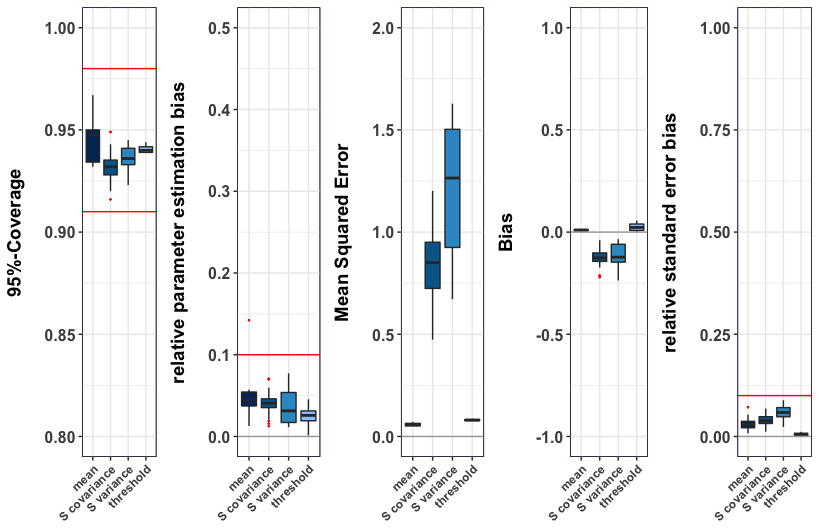
\includegraphics[width=1\textwidth]{Boxplot_LatentState_freeSvar_5categ.png}
   \end{center}
    \end{adjustwidth}
      \captionsetup{skip=10pt,width=1.05\textwidth}
\caption[Results LS 5 categ]{Results of the simulation study for the Latent State (LS) model including one construct with freely estimated latent State variances and covariances, spanning 9 measurement time points. Ordinal indicators were simulated with 5 ordered categories. Boxplots display the distribution of the respective statistic across different parameters of the same parameter type.}
\label{Fig: LS one free 5 categ}
\end{figure}

  \subsubsection{Freely varying state variances and covariances across time points. 7 ordered categories.}
  
 \begin{figure}[H]
 \begin{adjustwidth}{-1cm}{-1cm}
    \begin{center}
  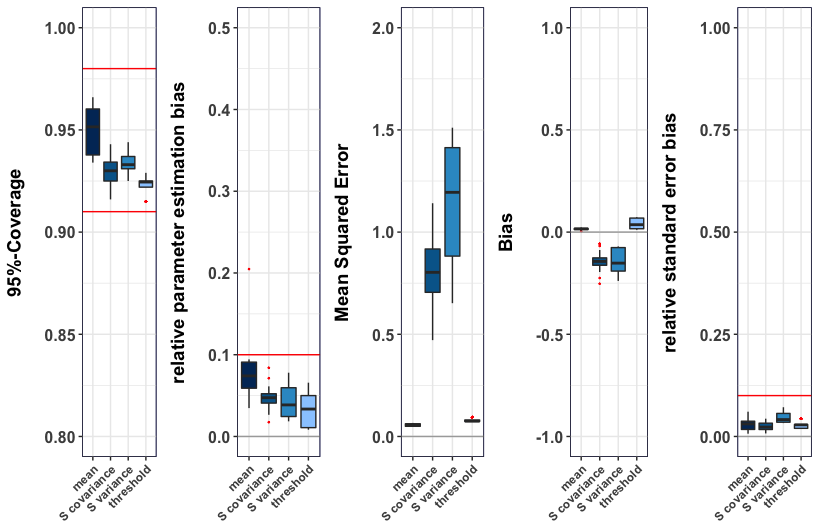
\includegraphics[width=1\textwidth]{Boxplot_LatentState_freeSvar_7categ.png}
   \end{center}
    \end{adjustwidth}
      \captionsetup{skip=10pt,width=1.05\textwidth}
\caption[Results LS 7 categ]{Results of the simulation study for the Latent State (LS) model including one construct with freely estimated latent State variances and covariances, spanning 9 measurement time points. Ordinal indicators were simulated with 7 ordered categories. Boxplots display the distribution of the respective statistic across different parameters of the same parameter type.}
\label{Fig: LS one free 7 categ}
\end{figure}


\subsection{Latent State Trait models: One construct}
  \subsubsection{Fixed state variances across time points. Default priors.}

 \begin{figure}[H]
 \begin{adjustwidth}{-1cm}{-1cm}
    \begin{center}
  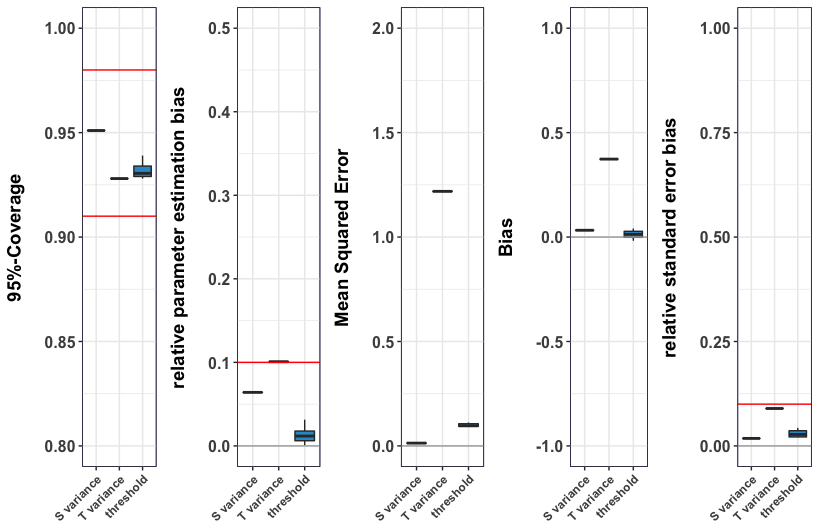
\includegraphics[width=1\textwidth]{Boxplot_LST_fixed.png}
   \end{center}
    \end{adjustwidth}
      \captionsetup{skip=10pt,width=1.05\textwidth}
\caption[Results LST fixed variance]{Results of the simulation study for the Latent State Trait (LST) model including one construct with latent state residual variances fixed to be equal across time, spanning 9 measurement time points. MPlus default priors. Ordinal indicators were simulated with 7 ordered categories. Boxplots display the distribution of the respective statistic across different parameters of the same parameter type.}
\label{Fig: LST one fixed}
\end{figure}


  \subsubsection{Fixed state variances across time points. Inverse gamma priors.}

 \begin{figure}[H]
 \begin{adjustwidth}{-1cm}{-1cm}
    \begin{center}
  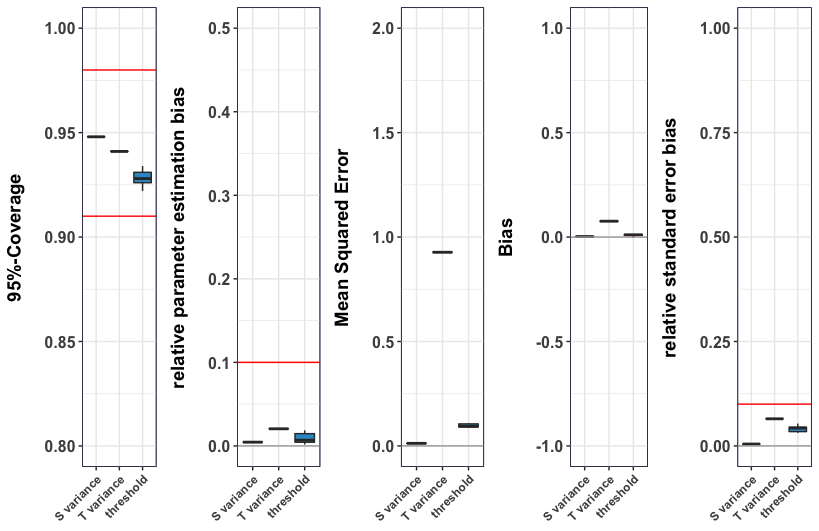
\includegraphics[width=1\textwidth]{Boxplot_LST_fixed_IGprior.png}
   \end{center}
    \end{adjustwidth}
      \captionsetup{skip=10pt,width=1.05\textwidth}
\caption[Results LST fixed variance IG]{Results of the simulation study for the Latent State Trait (LST) model including one construct with latent state residual variances fixed to be equal across time, spanning 9 measurement time points. Inverse gamma priors IG(0.001,0.001) for all variances. Ordinal indicators were simulated with 7 ordered categories. Boxplots display the distribution of the respective statistic across different parameters of the same parameter type.}
\label{Fig: LST one fixed IG}
\end{figure}


  \subsubsection{Free state variances across time points. Default priors.}


 \begin{figure}[H]
 \begin{adjustwidth}{-1cm}{-1cm}
    \begin{center}
  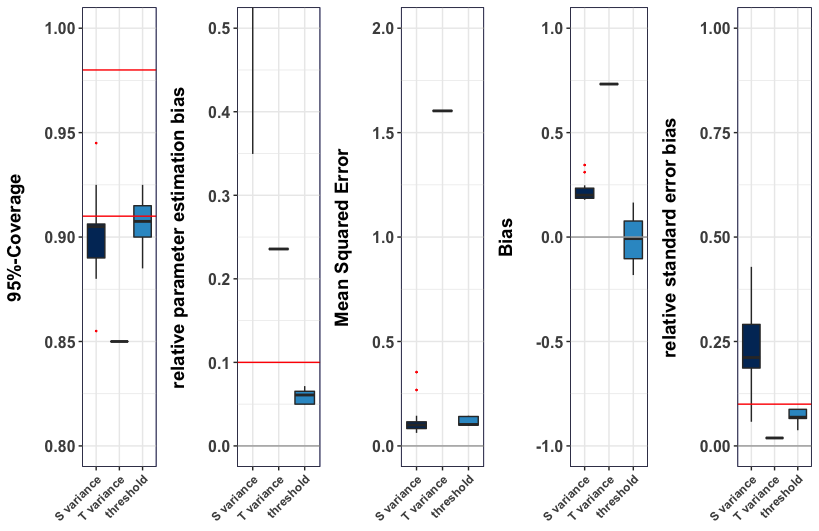
\includegraphics[width=1\textwidth]{Boxplot_LST_free.png}
   \end{center}
    \end{adjustwidth}
      \captionsetup{skip=10pt,width=1.05\textwidth}
\caption[Results LST free variance]{Results of the simulation study for the Latent State Trait (LST) model including one construct with latent state residual variances freely estimates across time, spanning 9 measurement time points.  Ordinal indicators were simulated with 7 ordered categories. Boxplots display the distribution of the respective statistic across different parameters of the same parameter type.}
\label{Fig: LST one free}
\end{figure}

  \subsubsection{Free state variances across time points. Inverse gamma priors.}

 \begin{figure}[H]
 \begin{adjustwidth}{-1cm}{-1cm}
    \begin{center}
  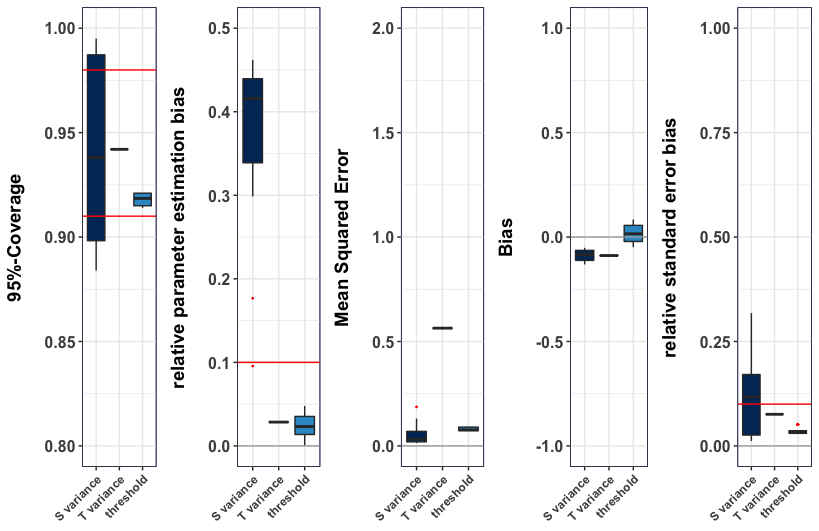
\includegraphics[width=1\textwidth]{Boxplot_LST_free_IGprior.png}
   \end{center}
    \end{adjustwidth}
      \captionsetup{skip=10pt,width=1.05\textwidth}
\caption[Results LST free variance IG]{Results of the simulation study for the Latent State Trait (LST) model including one construct with latent state residual variances freely estimates across time, spanning 9 measurement time points. Inverse gamma priors IG(0.001,0.001) for all variances. Ordinal indicators were simulated with 7 ordered categories. Boxplots display the distribution of the respective statistic across different parameters of the same parameter type.}
\label{Fig: LST one free IG}
\end{figure}

\subsection{Latent State models: Two constructs}
 \subsubsection{Free state variances and covariances across time points. Default priors.}

 \begin{figure}[H]
 \begin{adjustwidth}{-1cm}{-1cm}
    \begin{center}
  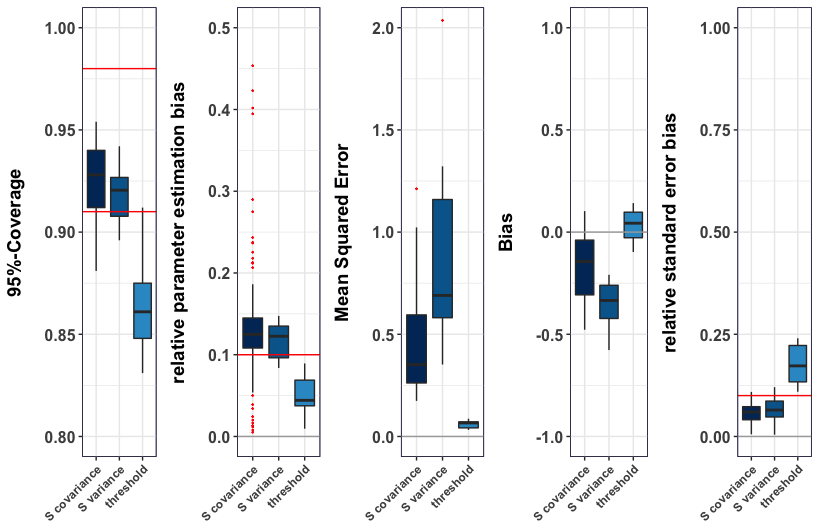
\includegraphics[width=1\textwidth]{Boxplot_Latent_State_2construcs_free.png}
   \end{center}
    \end{adjustwidth}
      \captionsetup{skip=10pt,width=1.05\textwidth}
\caption[Results LS free variance two constructs]{Results of the simulation study for the Latent State model including two constructs with latent state variances freely estimates across time, spanning 9 measurement time points.  Ordinal indicators were simulated with 7 ordered categories. Boxplots display the distribution of the respective statistic across different parameters of the same parameter type.}
\label{Fig: LS free}
\end{figure}

\subsection{Latent State Trait models: Two constructs}

 \subsubsection{Free state variances and covariances across time points.}
 
  \begin{figure}[H]
 \begin{adjustwidth}{-1cm}{-1cm}
    \begin{center}
  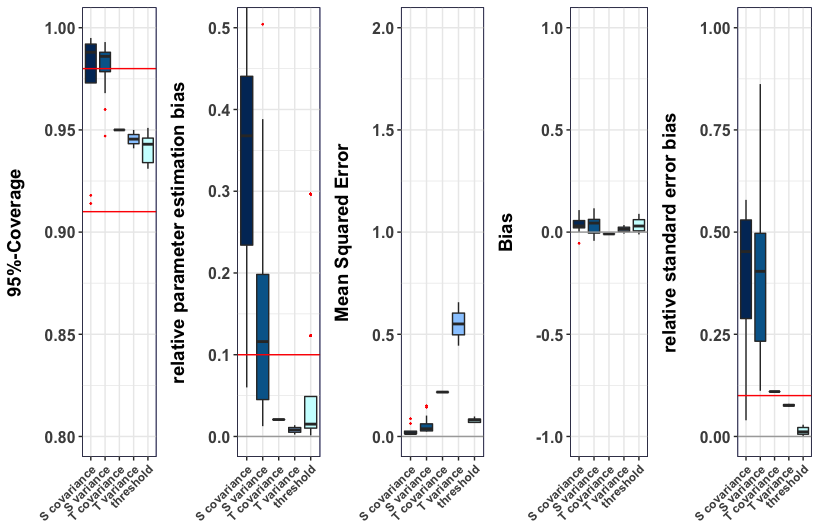
\includegraphics[width=1\textwidth]{Boxplot_LST_2constructs_freeSvar.png}
   \end{center}
    \end{adjustwidth}
      \captionsetup{skip=10pt,width=1.05\textwidth}
\caption[Results LST free variance two constructs]{Results of the simulation study for the Latent State Trait (LST) model including two constructs with free latent state residual variances across time, spanning 9 measurement time points.  Ordinal indicators were simulated with 7 ordered categories. Boxplots display the distribution of the respective statistic across different parameters of the same parameter type.}
\label{Fig: LST two free}
\end{figure}


 \subsubsection{Fixed state variances and covariances across time points.}

 \begin{figure}[H]
 \begin{adjustwidth}{-1cm}{-1cm}
    \begin{center}
  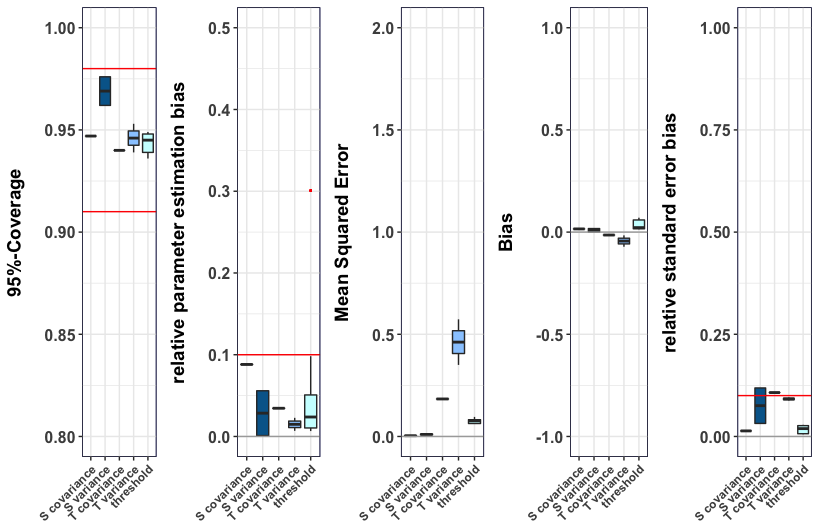
\includegraphics[width=1\textwidth]{Boxplot_LST_2constructs_fixed.png}
   \end{center}
    \end{adjustwidth}
      \captionsetup{skip=10pt,width=1.05\textwidth}
\caption[Results LST fixed variance two constructs]{Results of the simulation study for the Latent State Trait (LST) model including two constructs with fixed latent state residual variances across time, spanning 9 measurement time points.  Ordinal indicators were simulated with 7 ordered categories. Boxplots display the distribution of the respective statistic across different parameters of the same parameter type.}
\label{Fig: LST two fixed}
\end{figure}


